\documentclass[UTF8,a4paper,12pt]{ctexbook} 

\usepackage{graphicx}%学习插入图
\usepackage{verbatim}%学习注释多行
\usepackage{booktabs}%表格
\usepackage{geometry}%图片
\usepackage{amsmath}
\usepackage{amssymb}
\usepackage{listings}%代码
\usepackage{xcolor}  %颜色
\usepackage{enumitem}%列表格式
\setenumerate[1]{itemsep=0pt,partopsep=0pt,parsep=\parskip,topsep=5pt}
\setitemize[1]{itemsep=0pt,partopsep=0pt,parsep=\parskip,topsep=5pt}
\setdescription{itemsep=0pt,partopsep=0pt,parsep=\parskip,topsep=5pt}
\usepackage{tcolorbox}
\usepackage{algorithm}  %format of the algorithm
\usepackage{algorithmic}%format of the algorithm
\usepackage{multirow}   %multirow for format of table
\usepackage{tabularx} 	%表格排版格式控制
\usepackage{array}	%表格排版格式控制
\usepackage{hyperref} %超链接 \url{URL}
\usepackage{tikz}
\usepackage{dirtree}


\usetikzlibrary{intersections,
	positioning,
	petri,
	backgrounds,
	fit,
	decorations.pathmorphing,
	arrows,
	arrows.meta,
	bending,
	calc,
	intersections,
	through,
	backgrounds,
	shapes.geometric,
	quotes,
	matrix,
	trees,
	shapes.symbols,
	graphs,
	math,
	patterns,
	external}
\CTEXsetup[format+={\flushleft}]{section}

%%%% 设置图片目录
\graphicspath{{figure/}}

%%%% 段落首行缩进两个字 %%%%
\makeatletter
\let\@afterindentfalse\@afterindenttrue
\@afterindenttrue
\makeatother
\setlength{\parindent}{2em}  %中文缩进两个汉字位

%%%% 下面的命令重定义页面边距,使其符合中文刊物习惯 %%%%
\addtolength{\topmargin}{-54pt}
\setlength{\oddsidemargin}{0.63cm}  % 3.17cm - 1 inch
\setlength{\evensidemargin}{\oddsidemargin}
\setlength{\textwidth}{14.66cm}
\setlength{\textheight}{24.00cm}    % 24.62

%%%% 下面的命令设置行间距与段落间距 %%%%
\linespread{1.4}
\setlength{\parskip}{0.5\baselineskip}
\geometry{left=1.6cm,right=1.8cm,top=2cm,bottom=1.7cm} %设置文章宽度
\pagestyle{plain} 		  %设置页面布局

%代码效果定义
\definecolor{mygreen}{rgb}{0,0.6,0}
\definecolor{mygray}{rgb}{0.5,0.5,0.5}
\definecolor{mymauve}{rgb}{0.58,0,0.82}
\lstset{ %
	backgroundcolor=\color{white},   % choose the background color
	basicstyle=\footnotesize\ttfamily,      % size of fonts used for the code
	%stringstyle=\color{codepurple},
	%basicstyle=\footnotesize,
	%breakatwhitespace=false,         
	%breaklines=true,                 
	%captionpos=b,                    
	%keepspaces=true,                 
	%numbers=left,                    
	%numbersep=5pt,                  
	%showspaces=false,                
	%showstringspaces=false,
	%showtabs=false,        
	columns=fullflexible,
	breaklines=true,                 % automatic line breaking only at whitespace
	captionpos=b,                    % sets the caption-position to bottom
	tabsize=4,
	commentstyle=\color{mygreen},    % comment style
	escapeinside={\%*}{*)},          % if you want to add LaTeX within your code
	keywordstyle=\color{blue},       % keyword style
	stringstyle=\color{mymauve}\ttfamily,     % string literal style
	frame=single,
	rulesepcolor=\color{red!20!green!20!blue!20},
	% identifierstyle=\color{red},
	language=c++,
}
 \author{\kaishu 郑华}
 \title{\heiti U3D笔记}
 
\begin{document}          %正文排版开始
 	\maketitle

\chapter{基础}
	\url{https://unity3d.com/cn/learn/tutorials}
	
	\section{Scene 场景- 世界变换}	
	
	\section{Console 调试信息 - Crtl+Shift+C}
	
	\section{如何将脚本与具体对象绑定}
	
		\begin{enumerate}
			\item 右键\verb|asset|文件夹,创建C\#脚本
			\item 编写脚本
			\item 将\verb|asset |中的脚本拖拽到 \verb|hiearch |视图中的\verb|MainCamera |中
			\item 如果脚本是作用于场景中的某个物体,\textbf{则将该脚本拖拽到该物体上}
		\end{enumerate}
	
	\section{序列化-  [SerializedField]}
		\textit{通常情况下},GameObject上挂的MonoBehaviour脚本中的\textbf{私有变量}\textit{不会显示在Inspector面板上},即不会被序列化。
		
		\textbf{但如果指定了SerializedFiled特性},就可以被序列化了。
		
		\begin{lstlisting}
	public class Test : MonoBehaviour 
	{
		public string Name;
		[SerializeField]
		private int Hp; 
	}
		\end{lstlisting}
		
		\begin{figure}[H]
			\centering
			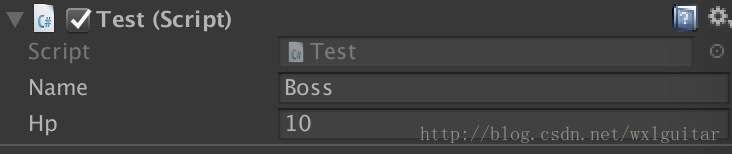
\includegraphics[scale=0.8]{SerilizedFiled.jpg}
			\caption{序列化操作 -在Inspector上显示}
		\end{figure}
	
	\section{常用技巧}
		\begin{itemize}
			\item \verb|ctrl + d| 复制
			\item \verb|shift + 鼠标 | 等比例缩放 
			\item \verb|shift + alt + 鼠标 | 原地等比例缩放
			\item \verb|在Unity 编辑器中输入汉字 | 需要借助其他文本拷贝粘贴
			\item \verb|q、w、e、r、t |在操作UI时尽量使用 T,以避免z轴发生的变化 
		\end{itemize}
	
\chapter{事件}
	\section{必然事件}
		继承自\verb|MonoBehaviour 类|后,自动会\textbf{按序}\textit{提供以下方法}:
		
		\begin{itemize}
			\item \verb|Awake()|:在加载场景时运行,用于在游戏开始前完成变量初始化、以及游戏状态之类的变量。
			\item \verb|Start()|:在第一次启动游戏时执行,用于游戏对象的初始化,在\verb|Awake() |函数之后。
			\item \verb|Update()|:是在每一帧运行时必须执行的函数,用于更新场景和状态。
			\item \verb|FixedUpdate()|:与\verb|Update() |函数相似,但是在固定的物理时间后间隔调用,用于物理状态的更新。
			\item \verb|LateUpdate()|:是在\verb|Update() |函数执行完成后再次被执行的,有点类似收尾的东西。 
		\end{itemize}
			
	\section{碰撞事件}
		U3D 的碰撞检测。具体分为三个部分进行实现,碰撞发生进入时、碰撞发生时和碰撞结束,理论上不能穿透
		
		\begin{itemize}
			\item \verb|OnCollisionEnter(Collision collision)| 当碰撞物体间刚接触时调用此方法
			\item \verb|OnCollisionStay(Collision collision)| 当发生碰撞并保持接触时调用此方法
			\item \verb|OnCollisionExit(Collision collision)| 当不再有碰撞时,既从有到无时调用此函数
		\end{itemize}

	\section{触发器事件}
		类似于 红外线开关门, 有个具体的范围,然后进入该范围时,执行某种动作,离开该范围时执行某种动作。类似于物体于一个透明的物体进行碰撞检测,理论上需要穿透,在U3D 中通过勾选 \verb|Is Trigger| 来确定该物体是可以穿透的。
		
		\begin{itemize}
			\item \verb|OnTriggerEnter() | 当其他碰撞体进入触发器时,执行该方法
			\item \verb|OnTriggerStay() | 当其他碰撞体停留在该触发器中,执行该方法
			\item \verb|OnTriggerExit() | 当碰撞体离开该触发器时,调用该方法
		\end{itemize}
		

\chapter{实体-人物、物体、组件}
	\section{实体类} \verb|GameObject 类|,游戏基础对象,用于填充世界。
		\paragraph{复制}
			\verb|Instantiate(GameObject)| 或 \verb|Instantiate(GameObject, position, rotation)|
			
			\begin{itemize}
				\item \verb|GameObject |指生成克隆的\textbf{游戏对象},也可以是\textbf{Prefab 的预制品}
				\item \verb|position |克隆对象的初始位置,类型为\verb|Vector3|
				\item \verb|rotation |克隆对象的初始角度,类型为\verb|Quaternion|
			\end{itemize} 
		
		\paragraph{销毁}
			\verb|Destroy(GameObject xx)- 立即销毁 |或 \verb|Destroy(GameObject xx, Time time)- 几秒后销毁|
			
		\paragraph{可见否}
			通过设置该参数调整该实体是否可以在游戏中显示,具体设置方法为\verb|gameObject.SetActive(true) 为可以显示,false 则隐藏|

		
	\section{获取实体上的组件}
		\paragraph{调用方式}\verb|GameObject.GetComponent<Type>().xx = xx;|
			
			\begin{itemize}
				\item \verb|cube1.GetComponent<RigidBody>().mass = 20;| //设置重量
				\item \verb|cube1.GetComponent<BoxCollider>().isTrigger = true;| //\textbf{开启Trigger 穿透方式}检测
				\item \verb|cube2.GetComponent<Test>().enable = false;| //\textbf{禁用Test脚本}
			\end{itemize}
	
	\section{物理作用实体类} \verb|Rigidbody 类|,一种特殊的游戏对象,该类对象可以在物理系统的控制下来运动。
		\paragraph{AddForce()}
			此方法调用时\verb|rigidBody.AddForce(1, 0, 0);|,会施加给刚体一个瞬时力,在力的作用下,会产生一个加速度进行运动。
			
		\paragraph{AddTorque()}
			给刚体添加一个扭矩。
			
		\paragraph{Sleep()}
			使得刚体进入休眠状态,且至少休眠一帧。类似于暂停几帧的意思,这几帧不进行更新、理论位置也不进行更新。
			
		\paragraph{WakeUp()}
			使得刚体从休眠状态唤醒。
		
\chapter{世界变换}
	\section{Transform 类}
		\paragraph{位置}
			transform.position = new Vector3(1, 0, 0);
		
		\paragraph{角度}
			transform.eulerAngles = new Vector3(x, y, z);
		
		\paragraph{旋转}	
			transform.Rotate(x, y, z);
			 
		\paragraph{缩放}
			transform.localScale(x, y, z); // 基准为1、1、1, 数为缩放因子。
			
		\paragraph{平移}
			transform.Translate(x, y, z); 

	\section{注意}
		在变化的过程中需要乘以 Time.deltaTime ,否则会出现大幅不连贯的画面。

\chapter{键盘鼠标控制}
	\section{普通按键 -keyDown(KeyCode xx)}
		\paragraph{方式一}
		
			\begin{itemize}
				\item 定义按键码:\verb|KeyCode keycode;|
				\item 判断键是否被按下:\verb|if(Input.GetKeyDown(keycode)){}|
				\item 在\verb|Inspirit -> Keycode |指定关联按键
			\end{itemize}
	
		\paragraph{方式二}
			\begin{itemize}
				\item 在\verb|Update| 中更新添加如下代码
				\item \verb|if(Input.GetKeyDown(KeyCode.UpArrow))| 
				\item \verb|KeyCode.xx |包括了键盘所有的按键,常用的AWSD 如下 
					\begin{itemize}
						\item \verb|if (Input.GetKeyDown(KeyCode.S)) |
						\item \verb|if (Input.GetKeyDown(KeyCode.W)) |
					\end{itemize}
			\end{itemize}
		
	\section{根据输入设备 -getAxis()}
		参数分为两类: 
		\paragraph{一、触屏类}
		 	\begin{enumerate}
			 	\item \verb|Mouse X| 鼠标沿屏幕X移动时触发 
			 	\verb|Mouse Y| 鼠标沿屏幕Y移动时触发 
			 	\verb|Mouse ScrollWheel |鼠标滚轮滚动是触发 
		 	\end{enumerate}
			
			\begin{lstlisting}
	float mouseX = Input.GetAxis("Mouse X");
	float mouseY = Input.GetAxis("Mouse Y");
	
	transform.Rotate(Vector3.Up * mouseX * rotateSpeed); // 根据具体需求进行操作
			\end{lstlisting}
		
		\paragraph{二、键盘类}
		 	\begin{enumerate}
		 		\item Vertical 键盘按上或下键时触发 
		 		\item Horizontal 键盘按左或右键时触发
		 	\end{enumerate}
		 	
		 	\begin{lstlisting}
	float horizontal = Input.GetAxis("Horizontal");
	float vertical = Input.GetAxis("Vertical");
	
	Vector3 desPos = (transform.forward * vertical  + transform.right * horizontal) * Time.deltaTime * moveSpeed;
	
	_rigidBody.position += desPos;
		 	\end{lstlisting}
		\textbf{返回值}是一个数,正负代表方向
			
\chapter{时间}
 	\section{Time 类}
 		该类是 U3D 在游戏中获取时间信息的接口类。常用变量如下:
 		
 		\begin{table}[H]
 			\centering
 			\caption{时间变量对照表}
 			\begin{tabular}{m{4cm}|m{10cm}}
 				\toprule
 					变量名 & 意义\\
 				\midrule
 					time & 游戏从开始到现在的运行时间, 单位为秒\\
 					\verb|deltaTime|     & 从上一帧到当前帧消耗的时间 \\
 					fixedTime     & 最近FixedUpdate 的时间,从游戏开始计算 \\
 					\verb|fixedDeltaTime|     & 物理引擎和FixedUpdate 的更新时间间隔 \\
 					timeSceneLevelLoad     & 从当前Scene 开始到目前为止的时间 \\
 					realTimeSinceStartup     & 程序已经运行的时间 \\
 					\verb|frameCount|     & 已经渲染的帧的总数 \\
 				\bottomrule 
 			\end{tabular}
 		\end{table}
 		 		

\chapter{数学}
	\section{Random 类}
		随机数类
		
	\section{Mathf 类}
		数学类
		
\chapter{物理}
	\section{流程}
		\begin{itemize}
			\item \verb|RigidBody |:创建,以完成受力接收。
			\item \verb|Physical Material|:创建,以完成多种力的添加。
			\item \verb|Material |:拖入材质球。
		\end{itemize}

\chapter{烘培}
	\section{简介}
		只有静态场景才能完成烘培(Bake)操作,其目的是在游戏编译阶段完成光照和阴影计算,然后以贴图的形式保存在资源中,以这种手段避免在游戏运行中计算光照而带来的CPU和GPU损耗。
		
		\begin{itemize}
			\item \textbf{如果不烘培}:游戏运行时,这些阴影和反光是由CPU和GPU计算出来的。
			\item \textbf{如果烘焙}:游戏运行时,直接加载在编译阶段完成的光照和阴影贴图,这样就不用再进行计算,节约资源。
		\end{itemize}
	
	\section{流程}
	
	
\chapter{寻路}
	\section{简介}
		NPC 完成自动寻路的功能。
		
	\section{流程}
		\begin{itemize}
			\item 将静态场景调至(Navigation Static)
			\item 烘焙
			\item 添加 \verb|Navigation Mesh Agent| 寻路组件
			\item 在脚本中设置组件的目标地址,添加目标
		\end{itemize}
	
\chapter{UGUI}
	在脚本中使用时记得加上\verb|using UnityEngine.UI |
	
	\section{场景跳转- SceneManager}
		
	\section{锚点- 自适应屏幕}
		\begin{itemize}
			\item 定义摄像机观察原点
			\item 其他物体与 锚点(Anchor) 距离保持一致,因此随着屏幕的变化,其他UI组件与屏幕锚点的距离始终保持一致
			\item 每个物体都可以定义自己的锚点
		\end{itemize}
	
		\paragraph{锚点类型}
			\begin{itemize}
				\item 位置类型\verb| 左上角、中心等|
				\item 拉伸类型\verb| 纵向拉伸适配、横向、整体|
			\end{itemize}
		
	\section{按钮}
		\subsection{原始Button}
			
		\subsection{Image等 -添加button 组件}
			\begin{itemize}
				\item \verb|create -> UI -> Image|
				\item \verb|Inspirit -> Add Component -> button|
			\end{itemize}	
		
		\subsection{添加事件处理脚本}
			\begin{itemize}
				\item 书写脚本并添加到Button gameObject 上
				\item 如果是Button 组件的话直接在button 组件上添加,如果是Image 则添加button 组件后再添加
				\item  添加脚本对象到\verb|onClick() |部分:\verb|+ -> gameObject 拖进来  -> 选择脚本中的具体函数|
			\end{itemize}
		
	\section{文本- Text}
		\subsection{添加文字阴影 -shadow 组件}
			\verb|addComponent -> shadow|
			
		\subsection{添加文子边框 -outline 组件}
			\verb|addComponent -> outline|
			
	\section{图片- ImageView}
		
	\section{选中标记- Toggle}
		\paragraph{Toggle 基本}
		
		\paragraph{Toggle Group}
			\subparagraph{选项栏设定}
				将panel  拖入 toggle 中的\verb|value changed|部分
				
			\subparagraph{预设}
				确定默认打开哪个panel,然后将其\verb|IsOn| 勾选,其余取消勾选	
				
	\section{滚动区域、滚动条}
	
	
	\section{其他工具条}
	
	\section{布局- Layout}
		\begin{itemize}
			\item 具体页面下创建空物体 \verb| GameObject|
			\item 其次在\verb|GameObject 下|添加组件 \verb|-> grid layout group|
			\item 最后在这个\verb|GameObject |下创建出各种Image 组件,然后这些组件将会以\verb|grid layout| 的布局进行自动调整
		\end{itemize}
	
		\subsection{grid layout group}
			\begin{itemize}
				\item  调整\verb|cell size| 进行调整子物件的大小
				\item  \verb|cell size| 的改变只影响子组件的第一层,既最下面一层
			\end{itemize}
		
		\subsection{horizontal layout group}
		
		\subsection{vertical layout group}
		
		
\chapter{着色器渲染}

		    
\chapter{跨平台发布apk}
	\section{流程}
		\begin{itemize}
			\item 安装 JavaSDK、Android Studio 并在SDK manager 里添加对应的API包
			\item 在unity 中的\verb|edit |选项下的\verb|preferences|, 并选中\verb|External Tools| 选项,配置\verb|JDK |和\verb|Android SDK| 安装位置。
			\item 在unity 中的\verb|File -> Build Settings|中,添加需要添加的场景,并选择对应的平台(Android, IOS)等
			\item 在unity 中的\verb|Build Settings |中的\verb|Player Settings |设置以下几个重要内容。
				\begin{enumerate}
					\item \verb|Company Name |
					\item \verb|Product Name |
					\item \verb|Default Icon |:192$\times$192
					\item \verb|Default Orientation |
					\item \verb|Other Settings -> Identification |:修改为\verb|com.netease(Or Other).TestName(Or Other)|
				\end{enumerate}
		\end{itemize}	
	
	\section{Apk 安装常见错误}
		\url{http://mumu.163.com/2017/03/30/25905_680657.html}
			

		    
\end{document} 
 		    